\clearpage
\section{Discussion}
\label{sec:discussion}

The aim of this discussion is to embed the results and implications of our paper into the broader context of urban planning and accessibility.
We do so by first deriving implications from our results that are relevant to the city of Cologne, as well as, urban planning in general.
We then also discuss the limitations of our study and conclude by providing an outlook on future research.

\subsection{Interpretation of Results}
\label{subsec:interpretation_of_results}

In this section, we will derive quantitative and qualitative insights that based on our results.

\subsubsection{Runtime Observations}
We have shown that our method applies to a large city like Cologne, running in a reasonable amount of time on consumer hardware.
While the memory footprints may exceed 32 GB, using swap memory did not degrade the runtime beyond a reasonable amount.
This shows us two things:
First, we conclude that our method is efficient enough to be applicable to large cities.
Second, we see that the implementation of our method can be optimized further by reducing the memory footprint.
As the usage of swap memory does not significantly degrade the runtime, we know that either we keep unnecessary data in memory or that we are bound by CPU time, which can easily be fixed, as our method is parallelizable.
Therefore, we expect our method to scale well when using more powerful hardware or distributing the computation over multiple machines.
We have, therefore, successfully created a method that incorporates an arbitrary amount of transport modes while remaining computationally tractable, even for whole cities.

\subsubsection{Public Transport Effectiveness}
Our findings indicate that public transport effectively enhances accessibility, particularly in remote, low-POI-density suburban areas near high-frequency transport lines. 
However, it is costlier compared to bicycle sharing.
We summarize our findings for public transport effectiveness in the following inferences:
\begin{enumerate}
  \renewcommand{\labelenumi}{I\theenumi.}
  \item Public transport improves accessibility \label{item:pt_improves_accessibility}
  \item Public transport is more effective in remote areas than in the city's center \label{item:pt_effective_in_remote_areas}
  \item Public transport is more effective in areas with low accessibility than in areas with high accessibility  \label{item:pt_effective_in_areas_with_low_accessibility}
  \item Public transport is costlier than bicycle sharing \label{item:pt_costlier_than_bicycle_sharing}
\end{enumerate}
We will reiterate the findings in our results and show how they support the above inferences.
In Figure \ref{fig:mean_time_per_cost}, we can see that when users can afford a short public transport trip (cost of 2.20), their accessibility to POIs increases (I\ref{item:pt_improves_accessibility}).

% pt for areas of low accessibility 
The improvement seen by adding public transport mainly comes from areas with low accessibility, as seen in Table \ref{tab:optimal_x_minute_city_metric} and Figure \ref{fig:optimal_x_minute_city_metric} (I\ref{item:pt_effective_in_areas_with_low_accessibility}).
These areas, or hexagons, are likely far from POIs, and we suspect that public transport helps by covering these longer distances. 
However, adding public transport might not make a big difference in areas where it is already easy to get to these places. 
This is because using public transport often involves extra steps: walking to the bus or train stop and waiting for it to arrive. 
How much this extra time matters depends on the length of the trip.
For short trips, getting to and waiting for public transport could be a large part of the travel time, making it less valuable. 
Nevertheless, for longer trips, especially in the areas that were hard to reach before, this extra time is a smaller part of the journey. 
This makes public transport more beneficial for these longer trips. 

% pt better than a bicycle for 20% worst
In Figure \ref{fig:optimal_x_minute_city_metric}, we see the entire distribution of the optimal X-minute city metric for each scenario.
Notably, while public transport is worse than bicycle sharing for the 80\% most accessible hexagons, it shows a distinct advantage over bicycle sharing beyond the 80\% quantile, facilitating faster access in less accessible areas (I\ref{item:pt_effective_in_areas_with_low_accessibility}).
The reason for this change in effectiveness between public transport and bicycle sharing is most likely linked to how bicycle sharing is set up in Cologne. 
With most bicycles available in the city center's "Flex-Zone", suburban areas have fewer bicycles as they can only be found at stations.
Consequently, the least accessible hexagons, typically situated in suburban regions, experience low to no availability of bicycles, which explains the superiority of public transport in these areas. 

% rath/neumar is reachable better by pt
Inferences \ref{item:pt_effective_in_areas_with_low_accessibility} and \ref{item:pt_effective_in_remote_areas} are supported by comparing the optimal X-minute city metric spatially between public transport and bicycle sharing, as seen in Figure \ref{fig:bicycle_optimal_map} and \ref{fig:public_transport_optimal_map}.
We see the district of Rath/Neumar in the east, which shows low accessibility in general.
However, we can see that public transport has an advantage over bicycle sharing in this remote area.

% pt in hexagons with walking time above 15 minutes
When looking at Table \ref{table:hexagons_with_walking_time_above_15_minutes} we see that public transport can make 10\% of hexagons that are not valid in terms of the 15-minute city by walking alone, valid (\ref{item:pt_improves_accessibility}).
In addition, when looking at the spatial distribution of those hexagons in Figure \ref{fig:fixable_hexagons}, we see that the yellow hexagons, which are those that become valid in terms of the 15-minute city only through public transport, are primarily located outside the city in remote areas (I\ref{item:pt_effective_in_remote_areas}).

% pt only better at 90% Pareto front
In addition, when investigating the cost and X-minute city metric Pareto fronts in Figure \ref{fig:quantile_time_per_cost}, we see that public transport is only able to yield more significant improvements than bicycle sharing when considering only the 10\% worst accessible hexagons (I\ref{item:pt_effective_in_areas_with_low_accessibility}).

% cost stuff
Table \ref{tab:required_cost} and Figure \ref{fig:maximum_required_cost_for_x_minute_city} show that public transport's advantage at the least accessible hexagons comes at a cost (I\ref{item:pt_costlier_than_bicycle_sharing}).
As soon as the benefits of public transport manifest, the cost also increases to \euro{2.20}, which is obvious as public transport rides are always charged.
We can see, however, that it is rarely necessary to travel more than four stops, as the corresponding cost of \euro{3.20} is only reached for the few least accessible hexagons.
The different sub-scenarios can explain the three- or four-step increases to the cost of \euro{2.20} and \euro{3.20}.
In some scenarios, it might be only beneficial to use public transport later.

Looking at Figure \ref{fig:public_transport_cost_map} also clearly reveals the spatial usage pattern of public transport.
As already conjectured previously, we see that public transport is mainly used in remote locations outside the city, which we know have lower accessibility in general (I\ref{item:pt_effective_in_remote_areas} \& I\ref{item:pt_effective_in_areas_with_low_accessibility}).

The isolated hexagons inside the cities seen in Figure \ref{fig:maximum_required_cost_for_x_minute_city} are most likely located very close to a public transport stop, enabling residents to use the public transport system without any loss of time.
Inside the city, it seems only beneficial to use the public transport system to reach necessities when living near a stop.
However, outside the city, the larger groups of hexagons indicate that using the public transport system is often faster than walking to the necessities, even though walking to the next stop requires some time (I\ref{item:pt_effective_in_remote_areas}).
This may be because the density of the POIs is lower outside the city.

% comparison of usefulness of short and long trips (not assigned to inference)
With the help of the cost and X-minute city metric Pareto fronts, we can evaluate the usefulness and cost-efficiency of short trips (those that travel no more than four stops) and long trips (those that travel more than four stops).
Figure \ref{fig:mean_time_per_cost} and Table \ref{tab:differences_in_mean_pareto_front} show that the improvement caused by the short trip tickets is, on average, 1 minute and 17 seconds, compared to the 4 seconds of long trip tickets, and therefore almost 20 times larger.
Unlike what we previously inferred in I\ref{item:pt_effective_in_remote_areas}, the most effective and cost-efficient use of public transport consists of short trips.
However, we should note that just because it does not bring as much value to travel more than four stops, this does not mean that trips associated with four stops or fewer are short.
Especially in suburban areas, where public transport stops are more sparse than in the city center, it might very well be that trips with four stops or fewer still travel multiple kilometers.
When investigating the 25\% quantile and 75\% quantile Pareto fronts in Figure \ref{fig:quantile_time_per_cost}, there is no benefit of long-distance tickets displayed.
Only when investigating the 90\% quantile Pareto front is the benefit visible.
This indicates that long-distance trips are only used for the least accessible hexagons located outside the city \ref{item:pt_effective_in_remote_areas}.

% Rath/Neumar
In Figure \ref{fig:public_transport_optimal_map}, we see that while the district of Rath/Neumar shows bad accessibility for all three scenarios, the accessibility in the public transport is better than that of walking and bicycle sharing (I\ref{item:pt_effective_in_remote_areas}).
Also, we know that the high-frequency city train line 9 runs through this region, which explains the effectiveness of public transport in this region (I\ref{item:pt_effective_in_areas_with_low_accessibility}).
It also shows us that a high-frequency public transport line from the city center to less accessible areas can significantly improve accessibility.

\subsubsection{Bicycle Sharing Effectiveness}
% intro
Bicycle sharing enhances accessibility in less and well-connected urban areas, offering cost-efficiency over public transport, with its effectiveness highly depending on bicycle allocation.
We summarize our findings for bicycle sharing effectiveness in the following inferences:

\begin{enumerate}
  \renewcommand{\labelenumi}{I\theenumi.}
  \item Bicycle sharing improves accessibility \label{item:bicycle_improves_accessibility}
  \item Bicycle sharing can further improve accessibility in already well-connected areas \label{item:bicycle_improves_accessibility_in_well_connected_areas}
  \item Bicycle sharing is only effective in areas, where bicycles are available \label{item:bicycle_where_available}
  \item Bicycle sharing is more cost-efficient than public transport \label{item:bicycle_more_cost_efficient_than_pt}
\end{enumerate}

We will reiterate our results and show how they support the above inferences.
In Figure \ref{fig:mean_time_per_cost} we can see that when users can afford a bicycle for 15 minutes (cost of \euro{1}), their accessibility to POIs increases drastically (I\ref{item:bicycle_improves_accessibility}).

As detailed in Table \ref{tab:optimal_x_minute_city_metric} and Figure \ref{fig:optimal_x_minute_city_metric}, the introduction of bicycle sharing yields benefits across almost all hexagons, offering a more uniform impact compared to public transport (I\ref{item:bicycle_improves_accessibility}).
Notably, bicycle sharing also yields improvements in already well-accessible areas (I\ref{item:bicycle_improves_accessibility_in_well_connected_areas}).
We think this is because bicycles have a lower overhead than public transport, which contributes significantly to their practicality in urban settings.
Firstly, the higher density of bicycle access points compared to public transport stops inherently reduces the initial distance required to access a mode of transport, facilitating quicker access to the transport system. 
Secondly, bicycles eliminate the waiting period often associated with public transport schedules, which means that once a user reaches a bicycle, they can immediately start their journey. 
This immediacy and ease of access render bicycles an effective solution for a more general scope than public transport.

Further, the data in Figure \ref{fig:optimal_x_minute_city_metric} reveals that in more accessible hexagons, combining bicycles with public transport offers greater advantages over using public transport alone (I\ref{item:bicycle_improves_accessibility_in_well_connected_areas}).
Interestingly, looking at the least accessible hexagons, the disparity between these two scenarios narrows. 
This observation implies that in areas with very low accessibility, which are most likely remote areas, the addition of bicycles does not significantly enhance accessibility.
This trend is likely due to the limited availability of bicycles in these less accessible areas, underscoring the importance of equitable distribution in bicycle-sharing systems (I\ref{item:bicycle_where_available}).

We think the decrease in bicycle effectiveness in areas with low accessibility is linked to the low availability of bicycles in suburban areas, as most bicycles are located in the "Flex-Zone".
This hypothesis is supported when looking at the difference between Figures \ref{fig:bicycle_optimal_map} and \ref{fig:walking_optimal_map}. 
Here, an improvement is observed in the bicycle scenario compared to walking, particularly within the "Flex-Zone" as shown in Figure \ref{fig:flex_zones}, which underscores the impact of bicycle availability on its effectiveness (I\ref{item:bicycle_where_available}).
\begin{figure}
  \begin{center}
    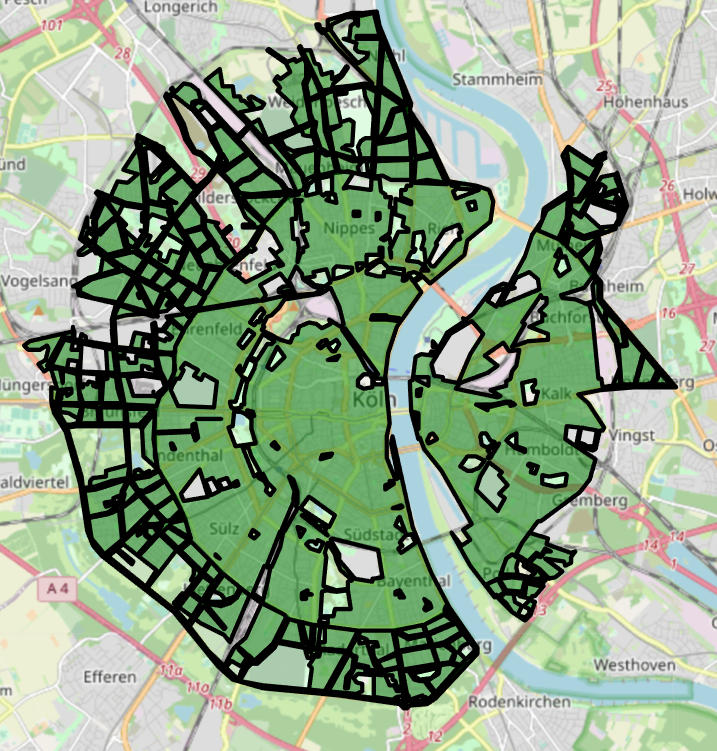
\includegraphics[width=0.50\textwidth]{Figures/discussion/flex_zones.png}
  \end{center}
  \caption{Next Bike's Flex Zones}
  \label{fig:flex_zones}
\end{figure}

Figure \ref{fig:problematic_hexagons} shows hexagons that are valid in terms of the 15-minute city by walking in green, those that are valid only by the addition of any sustainable mode of travel in yellow, and those that are not valid through any sustainable mode of travel in red.
We suspect that the very noticeable yellow ring around the city center is in an area with few POIs but still a high availability of bicycles, which can compensate for this sparsity.
This spatially shows where sustainable modes of travel are important to compensate for the sparsity of POIs.
These areas do not provide a close enough proximity to be considered sub-15-minute city regions by walking alone.
However, with bicycle sharing and public transport, they are.
In Figure \ref{fig:fixable_hexagons}, we see that most of the hexagons in the ring are orange or green, meaning they are either fixable by bicycle sharing or public transport.
This again underlines that bicycle sharing is more effective if it is present than public transport (I\ref{item:bicycle_where_available}\&I\ref{item:bicycle_improves_accessibility}).
In the same Figure, we can see that yellow hexagons, only fixable through public transport, tend to exist in the regions that are further away.
Also, the unfixable regions, marked in red,  mostly don't have bicycles near them, but they often have public transport stops nearby.
This suggests that bicycles are more effective than public transport in helping a region to become a sub 15-minute region (I\ref{item:bicycle_where_available}\&I\ref{item:bicycle_improves_accessibility}).

% pt only better at 90% Pareto front
Investigating the cost and X-minute city metric Pareto fronts in Figures \ref{fig:mean_time_per_cost} and \ref{fig:quantile_time_per_cost}, as well as, the corresponding steps in Tables \ref{tab:differences_in_mean_pareto_front}, \ref{tab:differences_in_75_quantile_pareto_front} and \ref{tab:differences_in_90_quantile_pareto_front} shows that using a bicycle for 15 minutes always yields more significant time gains than public transport except for the 10\% worst accessible hexagons (I\ref{item:bicycle_improves_accessibility} \& I\ref{item:pt_costlier_than_bicycle_sharing}).
This is a clear indicator of the superiority of bicycle sharing over public transport in terms of accessibility improvements, especially, when considering that the bicycle-sharing infrastructure does not cover all of the considered area.

% cost stuff
Table \ref{tab:required_cost} and Figure \ref{fig:maximum_required_cost_for_x_minute_city} show that bicycle sharing never costs more than public transport if both are used (\ref{item:bicycle_more_cost_efficient_than_pt}).
We can also deduct this from the price of both and the fact that bicycles are never used for more than 15 minutes.
We know that bicycles are never used for more than 15 minutes as the maximum cost, as seen in Table \ref{tab:required_cost}, is \euro{1}, which is the price for a 15-minute ride.
Meanwhile, the shortest possible public transport trip costs \euro{2.20}, as soon as public transport is used, it always costs more than bicycles.
Nevertheless, this shows that bicycle sharing is cheaper than public transport. 

In addition, knowing that bicycles are never used for more than 15 minutes tells us that at any location where bicycles are available, Cologne is a 15-minute city.
This is a strong indicator that bicycle sharing can make regions 15-minute city regions, improving accessibility (I\ref{item:bicycle_improves_accessibility}).

Table \ref{tab:differences_in_mean_pareto_front} shows the average improvements of the X-minute city metric, at the steps in the Pareto front.
We see that bicycle sharing is, on average, more than three times more cost-efficient than public transport (I\ref{item:pt_costlier_than_bicycle_sharing}).
Further, investigating the differences at the 75\% and 90\% quantile Pareto fronts in Table \ref{tab:differences_in_75_quantile_pareto_front} and \ref{tab:differences_in_90_quantile_pareto_front}, shows that bicycle sharing always is more cost-efficient than public transport.

Table \ref{table:hexagons_with_walking_time_above_15_minutes} shows that bicycle sharing enables 13\% of hexagons, which are not sub-15-minute city regions by walking alone, to become accessible within this time frame. 
This improvement is more significant than that achieved by public transport.
% This shows that bicycle sharing is more effective than public transport (\ref{item:bicycle_improves_accessibility}).

Looking at the spatial distribution of those hexagons in Figure \ref{fig:fixable_hexagons}, we see that the orange hexagons, which are those that become valid in terms of the 15-minute city only through bicycle sharing, are mostly located at the city's border, where the "Flex-Zone" is still active.
This again shows that the effectiveness of bicycle sharing highly depends on the "Flex-zone" (\ref{item:bicycle_where_available}).


%END

% not sure where to put this
% Another difference between bicycles and public transport is that they differ notably in their speed and route flexibility. 
% Public transport typically travels faster than bicycles, which offers a clear advantage for covering long distances. 
% This speed is particularly beneficial when some POIs are far away, as public transport can effectively bridge these larger gaps. 
% However, the fixed routes of public transport mean that users may not always disembark close to their desired POI. 
% In contrast, bicycles offer the flexibility of route choice, allowing users to tailor their journey to arrive nearer to the POI. 
% This also aligns with the finding that public transport tends to be most effective for the least accessible hexagons, where distance to POIs is a significant factor.

% end


\subsubsection{Bicycle Sharing and Public Transport - Substitutes or Complements?}
% introduction of substitutional effects and complement I & II
As mentioned, we found clear evidence that bicycle sharing and public transport positively affect accessibility according to the X-minute city metric.
It is, however, not clear whether these modes are substitutional to each other, meaning that one mode can compensate for the other or whether they are complements.
We could potentially observe two sorts of complementary effects.
\begin{enumerate}
  \renewcommand{\labelenumi}{Complement \theenumi.}
  \item Bicycle sharing and public transport are effective under different circumstances and in different areas \label{item:different_circumstances}
  \item Bicycle sharing and public transport used together is necessary to improve accessibility \label{item:used_together}
\end{enumerate}
The presence of complement \ref{item:different_circumstances} means that one mode cannot replace the other, and each is necessary under specific circumstances.
The presence of complement \ref{item:used_together} means that both modes must be used together in a single journey to achieve the highest accessibility.
Both effects are not mutually exclusive, meaning we can observe both simultaneously.

Our results show evidence for both effects, yet complement \ref{item:different_circumstances} is more pronounced.
We will now reiterate our results and show how they support the complements above.

Table \ref{tab:optimal_x_minute_city_metric} shows that the combined scenario on average yields better accessibility than bicycle sharing and public transport alone.
This suggests that either complement I or complement II must be present.
We see evidence for complement I in the observation that bicycle sharing is most effective for the 80\% more accessible hexagons, while public transport is mostly only effective for the 20\% least accessible hexagons.
Table \ref{table:hexagons_with_walking_time_above_15_minutes} shows how many hexagons in which people are not able to reach all necessities in 15 minutes by walking can reach all necessities in under 15 minutes by public transport or bicycle sharing.
We see that bicycle sharing and public transport alone are equally important, as they fix 13\% and 11\% of hexagons, respectively.
In addition, a lot more hexagons are fixed by only one of them (24\%) than by either (7\%).
This again suggests that complement I is present.
However, figure \ref{fig:maximum_required_cost_for_x_minute_city} contradicts complement I, as we see that the combined mode has higher costs earlier, surpassed by public transport, only to be surpassed again by the combined mode.
We think that this contradicts complement I as the public transport costs surpass those of the combined mode, which suggests that public transport can be substituted by bicycle sharing to some degree.
%TODO explain this better


% complement II
The only finding that suggests the presence of complement II can be found in table \ref{table:hexagons_with_walking_time_above_15_minutes}, which shows that the combined scenario fixes around 2\%.
However, compared to the effect that bicycle and public transport have alone, this is not very significant.
Nevertheless, we see that the effect of complement II is present.


% implications
The presence of complement I should make us aware that the effectiveness of either mode is highly dependent on the spatial circumstances of the region.
Some regions might benefit more from bicycle sharing, while others benefit more from public transport.
It is, therefore, necessary to analyze each region separately to maximize the positive effect of sustainable modes of travel.

% not sure where to put this "conclusion"
% Our findings conclude that enhancing bicycle availability in areas with low accessibility could yield significant benefits.
% Additionally, the observed dynamics suggest that bicycles are more advantageous in areas with low to medium accessibility, while public transport predominantly benefits the least accessible areas.
% This again indicates that bicycles and public transport serve complementary, rather than substitutable, roles in urban mobility networks.
% Therefore, removing one mode of transportation cannot be effectively compensated for by simply increasing the other, as each serves distinct and crucial functions in addressing different aspects of urban accessibility.


\subsubsection{Monetary Considerations}

Table \ref{tab:differences_in_mean_pareto_front} shows how a minute of saved time costs for cycling and public transport, respectively.
The most cost-efficient variant, bicycle sharing, enables users to save 1 minute and 40 seconds per euro, which might not be worth it for most people.
The 1.68 minutes per euro spent, in other words, means that to save a minute, people have to spend around 62 cents.
Comparing this to the minimum wage in Germany of \euro{12} per hour in 2022 \shortcite{federalstatisticalofficegermanyMinimumWages}, which is 20 cents per minute, shows that it takes around three minutes to make enough money to save one minute, which is obviously not worth it.
This means that, on average, the sustainable modes of travel are currently too expensive.

Even when looking at the least accessible regions (90\% quantile) separately in Figure \ref{fig:90_quantile_time_per_cost}, where we have the most significant improvement possible, the most cost-efficient mode of transport, which is bicycle, only yields an improvement of two minutes per euro, which again does not result in a net positive for people who earn the minimum wage.

With the help of the monthly cost depicted in Table \ref{tab:monthly_costs_per_scenario_15} and \ref{tab:monthly_costs_per_scenario_10}, we can derive recommendations for the price of a monthly ticket or subscription that is appealing to residents, that have to use public transport or bicycle sharing in order to reach certain amenities in under 10 or 15 minutes.
We expect that such a monthly ticket would reduce the cost of the trips necessary to reach the amenities to zero.
In our experiment in the city of Cologne, this is plausible, as the public transport tickets indeed allow for unlimited travel within the city, while NextBike's subscription makes trips that are under 30 minutes free.

Looking at the tables, we note that the monthly costs for the combined and bicycle scenarios are the same, which shows that only bicycle sharing is used in the combined scenario.
In the 15-minute benchmark, we see that in order to appeal to at least 50\% of the population, a public transport ticket should cost less than \euro{8.80}, while a bicycle sharing subscription should cost less than \euro{4}.
The 10-minute benchmark shows a similar pattern: the median cost for the bicycle and combined scenario is \euro{9}, while the median cost for the public transport scenario is \euro{19.80}.
Currently, a NextBike subscription costs \euro{10} per month, while the most common public transport ticket, the "Deutschlandticket", costs \euro{49} per month.
Both of these prices are significantly higher than the median cost for the bicycle and combined scenario, which means that a monthly ticket is not worth it for at least half of the affected hexagons.

Table \ref{tab:monthly_costs_for_cars} shows the monthly car cost, excluding acquisition costs.
With the difference between the monthly car cost and the monthly cost of the bicycle, combined and public transport scenario, we can calculate how significant acquisition costs for a car can be, so that it is still cheaper than the sustainable modes of travel.
In the case of the 15-minute benchmark, the average car costs are \euro{1.69}, while the average cost for the bicycle and combined scenario are \euro{5.79}, resulting in a difference of \euro{4.10} per month or \euro{49.20} per year.
This difference compared to the usual acquisition cost of a car is so low that it is not monetarily worth it to buy a car if the same journey can be made with bicycle sharing or public transport.
In addition, we have to keep in mind that our estimates for the speed of cars are very optimistic, as we assume that there is no traffic and that parking is always available.
Obviously, we can only state this for areas where accessibility using sustainable modes of travel suffices.
From table \ref{table:hexagons_with_walking_time_above_15_minutes}, we know that 67\% of hexagons in which walking alone is not sufficient, only cars can make all amenities accessible in under 15 minutes.


\subsubsection{Uncertainty}

The standard deviation of the average time it takes to reach all necessities for bicycles is 1 minute and 10 seconds. 
Relating this to the improvement compared to walking for 1 minute and 38 seconds, we see that the uncertainty is quite significant.
This shows us that bicycle placement significantly impacts the bicycle-sharing scenario's effectiveness (I\ref{item:bicycle_where_available}).

It is interesting to note that bicycles suffer more from uncertainty than public transport, as public transport only has a standard deviation of 16 seconds.
Relating the standard deviation to the improvement compared to walking of 1 minute and 28 seconds, it is less impactful than bicycles.
However, the standard deviation strongly depends on the choices of our sub-scenarios. 
For public transport, we tried 08:00, 12:00 and 18:00.
We suspect that the variance for public transport would increase more drastically and eventually surpass the one of bicycle sharing if we choose more unusual times like midnight.
In addition, the schedule of public transport is often the same for full hours.
We could get a more realistic picture by adding more times with non-zero minutes to our sub-scenarios.

We should also note that the comparison of variances should be taken with caution as the method for selecting the sub-scenarios differs per scenario.
We employed a clustering method for bicycle sharing while we made a qualitative choice for public transport. 

\subsection{Implications}
\label{sec:implications}

From our interpretation of the results, we can derive several implications for the city of Cologne and accessibility in cities in general.
We will structure our implications into two sections. First, we will discuss what already works well, and then we will discuss measures that can be taken to improve accessibility.

% What works well
What already works well is the improvement of accessibility through public transport in remote areas.
As long as there are areas with low accessibility caused by low availability of POIs, public transport will be an effective measure.
Also, bicycle sharing can improve accessibility everywhere where there are bicycles available.
For the most part, at least for Cologne, bicycle sharing is highly effective where the "Flex-Zone" is located.
It is essential to understand the relationship between its effectiveness and the location of this zone.
As most of Cologne's central parts are covered by the zone, we can already observe its massive positive effects on accessibility.
In addition, approximately 69\% of all considered hexagons and with that, 69\% of all residential in the administrative district Cologne ("Stadtkreis Köln") are 15-minute city by walking, which shows us that Cologne essentially already has excellent accessibility.
Interestingly, this \shortciteA{nicolettiDisadvantagedCommunitiesHave2023} calculated a vastly higher number. 

% improvements
% improvement 1: turning more non-15 minute regions into 15-minute regions
The observation that approximately 31\% of Cologne's area lacks access to essential services within a 15-minute walk highlights the potential for improvements.
We hypothesized that introducing bicycle sharing and enhanced public transport could significantly reduce these areas by improving accessibility.
However, as indicated in Table \ref{table:hexagons_with_walking_time_above_15_minutes}, a majority (67\%) of the hexagons currently not meeting 15-minute city criteria remain to not meet the criteria even with these sustainable modes.
Yet, it is important to note the impact of bicycles and public transport in converting 33\% of these hexagons into areas meeting the 15-minute city criteria.
To further amplify their effectiveness, we propose two strategies.
Firstly, expanding the 'flex zone' areas where bicycles are available into inaccessible regions. 
Given the observed correlation between bicycle availability and enhanced accessibility, this approach will likely yield substantial improvements.
Secondly, we recommend establishing high-frequency public transport lines to connect to remote, low-accessible areas. 
Our findings suggest that public transport effectively improves accessibility in these regions. 
However, considering the potential impracticality of extending the flex zone to these distant areas, adding or enhancing public transport routes could be a more feasible solution.

% improvement 2: effectively managing the bicycle-sharing fleet
We have demonstrated that the success of bicycle-sharing is closely tied to the availability of bicycles.
This availability primarily hinges on two factors: the location of the "Flex-zone" and how bicycles are distributed within it.
Significantly, our findings reveal that the program's effectiveness varies greatly across different sub-scenarios, highlighting the importance of strategic bicycle distribution.
Therefore, carefully managing bicycle placement and timely relocations are crucial for the system's efficiency.
To optimize the effectiveness of bicycle sharing, it is essential to conduct regular analyses of system demand and adjust bicycle distribution in response to these insights.
\shortciteA{heRobustRepositioningVehicle2020,luOptimizingProfitabilityQuality2018b,benjaafarDynamicInventoryRepositioning2018a} have already researched how to effectively relocate bicycles.

% TODO:
% improvement 3: reducing costs


% don't know what to do with this
% Merkenich & rhine bridge
% In Figure \ref{fig:optimal_map}, we observed that Merkenich, located on the other side of the Rhine next to Leverkusen, is one of the least accessible regions in Cologne.
% From Figure???, we know that there are plenty of POIs for all categories in Leverkusen, which are very close to the problematic region.
% This indicates a lack of mobility crossing the Rhine River.
% As a bridge already exists, we suggest providing a frequent public transport line to improve accessibility in Merkenich.

\subsection{Limitations}
\label{sec:limitations}

% This section shows the constraints and boundaries within which our current study on bicycle-sharing programs and urban accessibility operates.

% Exclusion of Traffic and Parking Factors

A significant limitation of our analysis is the omission of traffic conditions and parking availability. 
Urban traffic dynamics can significantly influence the practicality and speed of bicycles, especially car travel, potentially skewing the perceived efficiency.
Similarly, the availability of parking plays a crucial role in urban mobility, particularly in cities.
By not accounting for these factors, our study may not fully capture the complexities and challenges urban commuters face, possibly overestimating the effectiveness of bicycle-sharing and car travel in congested urban environments.

Another critical limitation is the exclusion of reliability issues such as public transport outages or traffic disruptions due to accidents. 
These events can drastically affect transportation dynamics in a city. 
For instance, a public transport outage might temporarily increase the demand for bicycles, while an accident could impede bicycle routes. 
Not considering these variables limits the scope of our study, particularly in understanding the resilience and adaptability of bicycle-sharing and public transport systems.

The usefulness of the X-minute-city metric employed in our study, which assesses accessibility based on the ability to reach any POI assigned to a category, should also be taken with caution.
For example, access to a pet doctor a health POI, is considered equivalent to access to a hospital.
While this metric provides a quantifiable measure of accessibility, it may not comprehensively represent the diverse needs of an urban population. 

In addition, our metric does not in any way consider the load of the POIs.
Consider, for example, a supermarket in the center of Cologne.
As the population density there is very high, the supermarket might be very crowded, effectively reducing its usefulness.
Conversely, a supermarket in a less dense area might be less crowded, making it more useful.
This insight should also be considered when using our method for planning purposes.

Our analysis also reveals a limitation concerning the scalability of transport modes. 
While bicycles significantly improve the X-minute city metric in our study, suggesting enhanced accessibility, they inherently lack the scalability of public transport. 
A bicycle may offer a convenient solution for an individual, but it does not address the mass transit needs of a larger population. 
This aspect is particularly crucial in dense urban areas where public transport systems are more efficient in moving large numbers of people. 
Therefore, while bicycles contribute to urban accessibility, they should be considered part of a broader, multi-modal transport strategy rather than a standalone solution.


\subsection{Future Work}
\label{sec:future_work}

Building upon the findings of our current study, it is essential to explore new avenues to deepen our understanding of urban mobility and enhance bicycle-sharing systems. 
This section outlines potential directions for future research that can contribute significantly to this field.

% Investigating Public Transport Disruptions
A crucial area of future research is examining the impact of public transport disruptions on accessibility.
Disruptions such as strikes, maintenance, or accidents can drastically alter commuting patterns. 
Investigating these scenarios could involve comparing accessibility between normal and disrupted conditions to determine the impact of outages and to what extent bicycle sharing or other modes can compensate for these outages.
This research can provide valuable insights into the role of bicycle-sharing as an alternative mode of transport during public transport failures.

% Flex Zone Enhancements
Another promising research direction is to study the effects of modifications to the flex zone. 
Changing the area where bikes can be borrowed and returned may significantly influence the accessibility improvements caused by bike-sharing. 
Future studies could experiment with different sizes and placements of flex zones to determine optimal configurations that maximize accessibility and efficiency.
These research endeavors should consider or even incorporate the dynamics of bicycle relocations.

% Improving Public Transport Lines
Investigating the impact of adding new or improving existing public transport lines on bicycle-sharing systems presents another research opportunity. 
Such a study could explore how enhancements in public transport affect accessibility in currently inaccessible areas.
Understanding these dynamics is crucial for integrated urban transport planning that caters to diverse commuter needs.

% Comprehensive Analysis of Transportation Usage
A comprehensive study on the usage patterns of roads, bicycles, and public transport is also essential. 
With the help of our current study, it is possible to find the paths people would take if they tried to get from one specific point to another.
This, together with realistic demand data, yields a set of paths that can be analyzed to find potential bottlenecks.
The results could inform urban planning and policy decisions, leading to more efficient and responsive urban transport systems.

While we managed to incorporate public transport and bicycle sharing, as well as, the combination of both, we did not consider all common modes of transport.
For example one might also consider personal bicycles, taxis, or e-scooters.

\subsection{Conclusion}
\label{sec:conclusion}
This thesis has explored the integration of bicycle sharing and public transport within the framework of the 15-minute city, focusing on their impact on urban accessibility in Cologne.
Our research demonstrates that while both bicycle sharing and public transport contribute to urban accessibility, their effectiveness varies based on location and mode.
Bicycle sharing shows pronounced benefits in central areas with high bicycle availability, while public transport is more advantageous in remote, less accessible areas.
A key finding is that these transportation modes are not entirely substitutable but rather complementary, each playing a unique role in enhancing urban accessibility under different circumstances.
Methodologically, the development of a new accessibility metric and routing algorithm represents a significant advancement in the field of urban planning, enabling the consideration of multiple transport modes and cost factors.
Our analysis reveals some limitations, such as the exclusion of traffic conditions and parking availability, which suggests avenues for future research. Addressing these limitations can lead to more robust and comprehensive urban planning strategies.
In conclusion, this thesis contributes to the understanding of multi-modal urban transportation systems, providing valuable insights for urban planners and policymakers in creating more accessible, efficient, and sustainable urban environments.

